
\section{Analiza systemu}

Celem projektu była analiza możliwości przetwarzania równoległego w architekturze czwórki z początkowymi danymi w dolnym węźle (jak pokazano na rysunku \ref{fig:schema}).
W ramach projektu zajmowaliśmy się dwoma modelami - sekwencyjnym oraz równoległym z jedną komunikacją na łączu.

\begin{figure}[!ht]
\centering
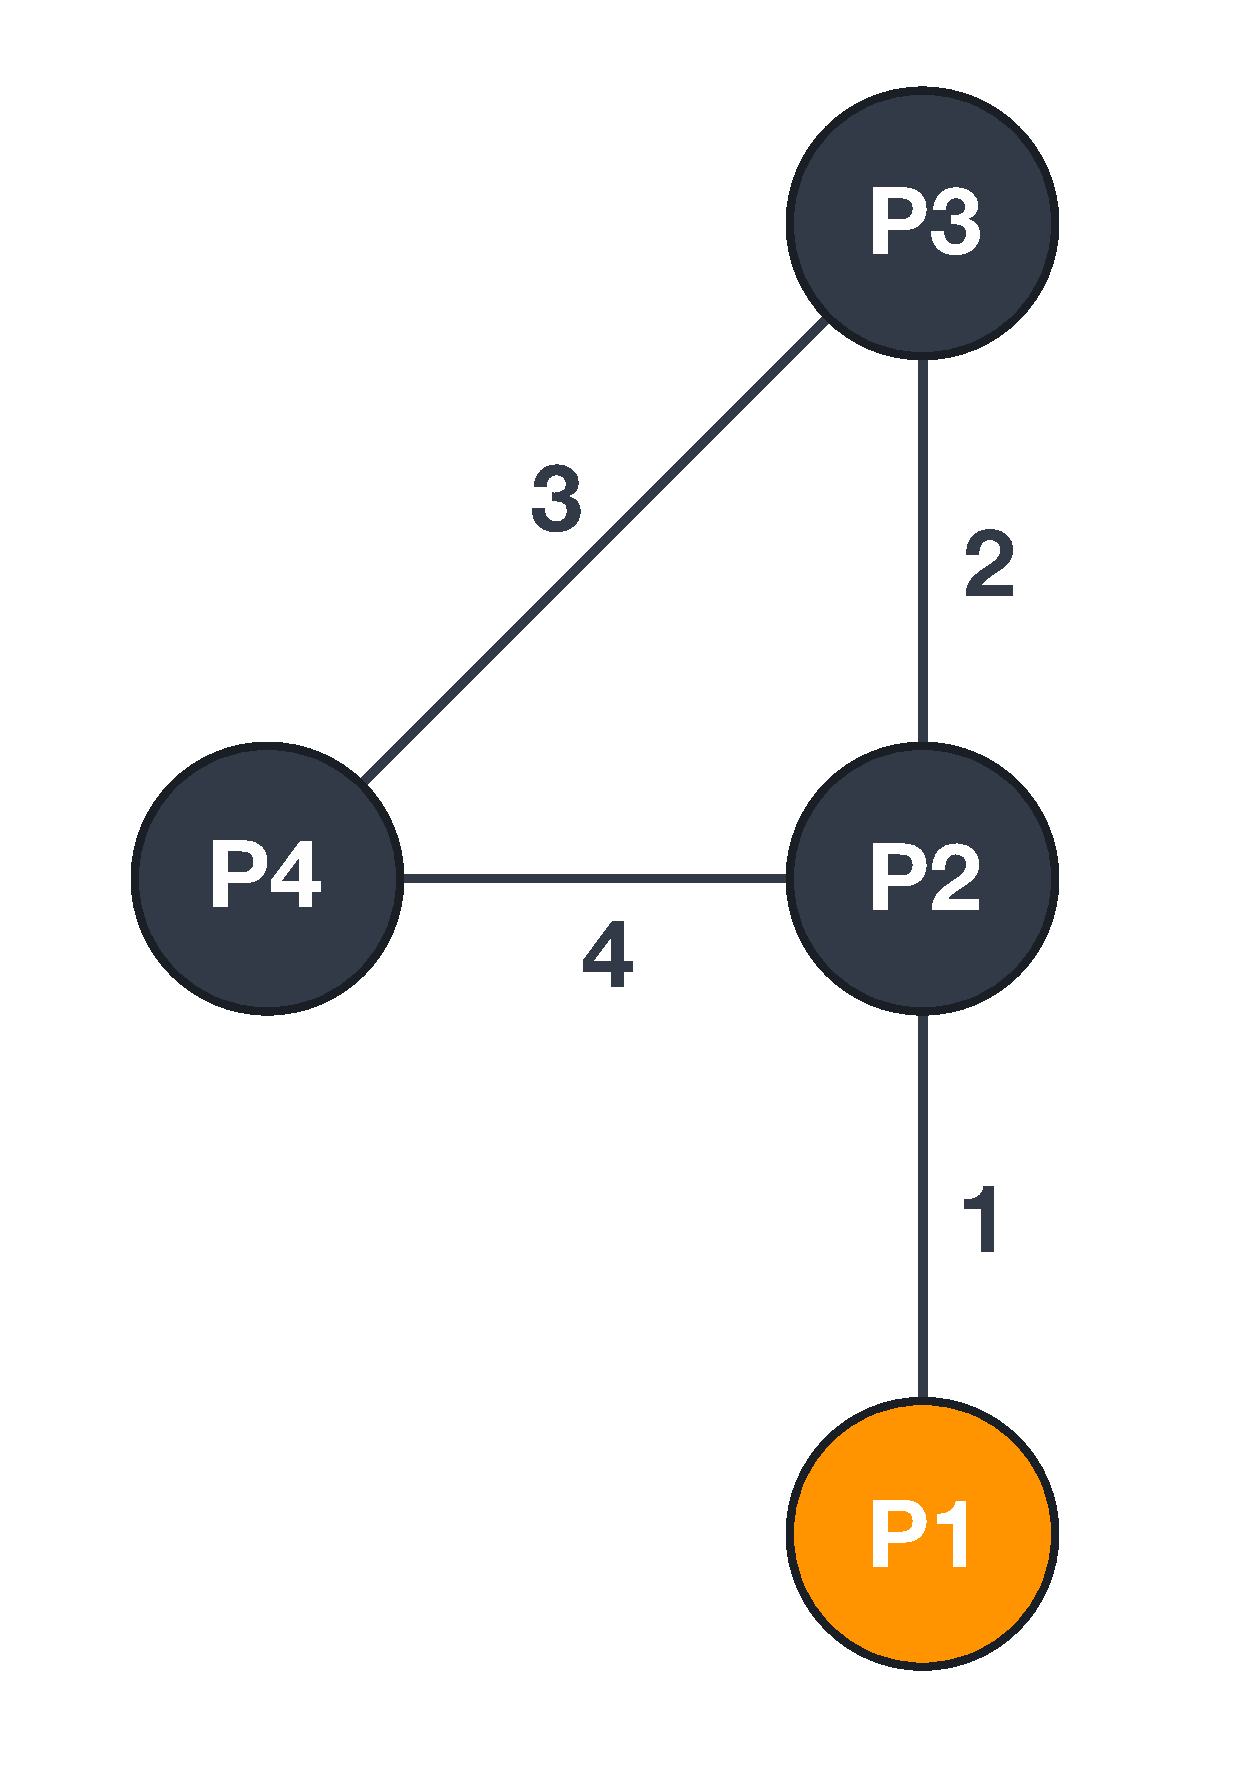
\includegraphics[width=0.5\textwidth]{schema.pdf}
\caption{Schemat systemu wraz z oznaczeniem procesorów}
\label{fig:schema}
\end{figure}

\subsection{Analiza modelu sekwencyjnego}

Analiza modelu sekwencyjnego.

\subsubsection{Pierwszy model sekwencyjny}

\subsubsection{Drugi model sekwencyjny}

\subsubsection{Trzeci model sekwencyjny}

\subsection{Analiza modelu równoległego}

Analiza modelu równoległego.

\subsubsection{Pierwszy model równoległy}

\subsubsection{Drugi model równoległy}

